\documentclass[journal]{IEEEtran}
\usepackage{filecontents}
\usepackage{cite}

\usepackage{colortbl}




\makeatletter
\def\endthebibliography{%
	\def\@noitemerr{\@latex@warning{Empty `thebibliography' environment}}%
	\endlist
}
\makeatother

\usepackage{stfloats}


\usepackage{url}
\hyphenation{op-tical net-works semi-conduc-tor}    

\title{Algoritmos de reconocimiento automático de patrones en computador de placa reducida para la detección de fibrilación auricular}

\author{
Claudia Ideth Céspedes Vigoya \\ %\IEEEauthorblockN{some author afiliation}
\and
Juan Calos Maya Gonzalez
\and

Oscar Fernando Avilés Sánchez

% \\ \IEEEauthorblockN{Servicio Nacional de Aprendizaje, Centro de Electriciad Electrónica y Telecomunicaciones}
}


\ifCLASSINFOpdf
\usepackage[pdftex]{graphicx}
%declare the path(s) where your graphic files are
%\graphicspath{{../pdf/}{../jpeg/}}
%and their extensions so you won't have to specify these with
%every instance of \includegraphics
%\DeclareGraphicsExtensions{.pdf,.jpeg,.png}
\else
%or other class option (dvipsone, dvipdf, if not using dvips). graphicx
%will default to the driver specified in the system graphics.cfg if no
%driver is specified.
\usepackage[dvips]{graphicx}
%declare the path(s) where your graphic files are
%\graphicspath{{../eps/}}
%and their extensions so you won't have to specify these with
%every instance of \includegraphics
%\DeclareGraphicsExtensions{.eps}
\fi
% graphicx was written by David Carlisle and Sebastian Rahtz. It is
% required if you want graphics, photos, etc. graphicx.sty is already
% installed on most LaTeX systems. The latest version and documentation
% can be obtained at: 
% http://www.ctan.org/pkg/graphicx
% Another good source of documentation is "Using Imported Graphics in
% LaTeX2e" by Keith Reckdahl which can be found at:
% http://www.ctan.org/pkg/epslatex
%
% latex, and pdflatex in dvi mode, support graphics in encapsulated
% postscript (.eps) format. pdflatex in pdf mode supports graphics
% in .pdf, .jpeg, .png and .mps (metapost) formats. Users should ensure
% that all non-photo figures use a vector format (.eps, .pdf, .mps) and
% not a bitmapped formats (.jpeg, .png). The IEEE frowns on bitmapped formats
% which can result in "jaggedy"/blurry rendering of lines and letters as
% well as large increases in file sizes.
%
% You can find documentation about the pdfTeX application at:
% http://www.tug.org/applications/pdftex
%


\usepackage[spanish]{babel}
\usepackage[utf8]{inputenc}


%\usepackage[backend=bibtex,style=ieee-alphabetic,natbib=true]{biblatex} %added
\usepackage[numbers]{natbib}
% \usepackage[authoryear,round,longnamesfirst]{nat}

\begin{document}
\title{Oximetría de Pulso Mediante Aplicación de Telemetría}
\maketitle


\begin{abstract}
	
El desarrollo de dispositivos que permitan la medición de la saturación parcial de oxígeno y su telemonitoreo en tiempo real implica, por un lado, la implementación de herramientas de procesamiento de las señales de fotopletismografìa; y por otro, la elaboración de códigos para el envío de la información y su gestión para garantizar su acceso en tiempo real. En el presente artículo se expone la elaboración de un sistema embebido microcontrolado que realiza el filtrado de las señales de fotopletismografìa entregadas por el sensor MAX30102, para a partir de la densidad espectral de potencia determinar los coeficientes relacionados con el cálculo de la saturación parcial de oxígeno. El telemonitoreo se realiza mediante un servidor web que recibe la información del sistema embebido para entregarla en tiempo real dado el acceso desde un explorador web. Se obtuvo una ejecución permanente en tiempo real y con valores medidos correlacionados con sensor de oximetría comercial (r=0.87) en saturaciones parciales de oxígeno superiores al 88\%. 


   
\end{abstract}
\IEEEpeerreviewmaketitle

\begin{IEEEkeywords}
	Saturación de oxígeno, MAX30102, fotopletismografía, embebido, densidad espectral de potencia, telemetría.
\end{IEEEkeywords}


\section{Introducción}



\IEEEPARstart{S}{e}gún la Organización Mundial de la Salud, las enfermedades no transmisibles son la principal causa de muerte, en 2012 fueron las causantes del 68\% del total de las muertes registradas \cite{A_OMS_informe}. Y entre estas enfermedades, las respiratorias crónicas ocupan el tercer lugar de prevalencia después de las enfermedades cardiovasculares y el cáncer, el 80\% de estas muertes ocurren en países de ingresos bajos y medios  %(A OMS prevención)%, 
\cite{A_OMS_prevencion}.

Los pacientes con enfermedades respiratorias crónicas se ven afectados en la cantidad de oxígeno en sangre por el reducido intercambio gaseoso alveolar. Para ellos, la medición de gases en sangre es el elemento principal en el diagnóstico y tratamiento \cite{A_webster_spo2}.  Al respecto, el oxímetro de pulso resulta ser la principal herramienta de uso clínico y de bajo costo que permite esta medición de manera no invasiva.

Por otro lado, el progresivo incremento de la expectativa de vida y de los riesgos asociados a enfermedades no transmisibles, enfatiza la importancia del cuidado de la salud en casa con la incorporación paulatina de diferentes tecnologías \cite{A_webster_home_care}. El objetivo es reducir el número de admisiones hospitalarias; permitiendo incluso, para la monitorización de signos vitales (como lo es la cantidad de oxígeno en sangre), el envío de información ininterrumpida a los profesionales de la salud. Este telemonitoreo permitirá evitar los errores de lectura y trascripción de los métodos actuales, como el de conexión de voz; y conllevará  a la incorporación de aplicaciones escalables en materia de alarmas automáticas e inteligencia artificial dada la cantidad de datos involucrada \cite{A_telemedicina}.

Desarrollar una herramienta tecnológica que permita el telemonitoreo de la cantidad de oxígeno en sangre implica abordar elementos propios de oximetría de pulso y de incorporación de aplicaciones que hacen uso de internet para garantizar la monitorización remota. Con respecto a la oximetría de pulso, se trata de hacer incidir una luz roja e infraroja (con diodos emisores de luz) sobre una estructura corporal y realizar la medición de la luz transmitida o reflejada en ambas longitudes de onda haciendo uso de fotodetectores (como fotodiodos). Dado el nivel de absorbancia diferencial entre hemoglobina oxigenada y sin oxigenar para cada una de las longitudes de onda, es posible determinar el porcentaje de oxígeno en sangre a partir de las señales leidas por el fotodetector (como  las que se indican en la figura \ref{principio_funcionamiento}), esto se logra con herramientas de procesamiento de señales para estimar características de las señales adquiridas.  Adicionalmente, con el oxímetro de pulso, por leer señales de voltaje pulsátiles (según el pulso del paciente), es factible realizar la medición de frecuencia cardíaca. Como resultado, después del procesamiento de la información,  los datos monitorizados en oximetría de pulso se componen de la siguiente información: porcentaje de saturación de oxígeno, frecuencia cardíaca y señales pletismográficas.

\begin{figure}[!h]
	\centering
	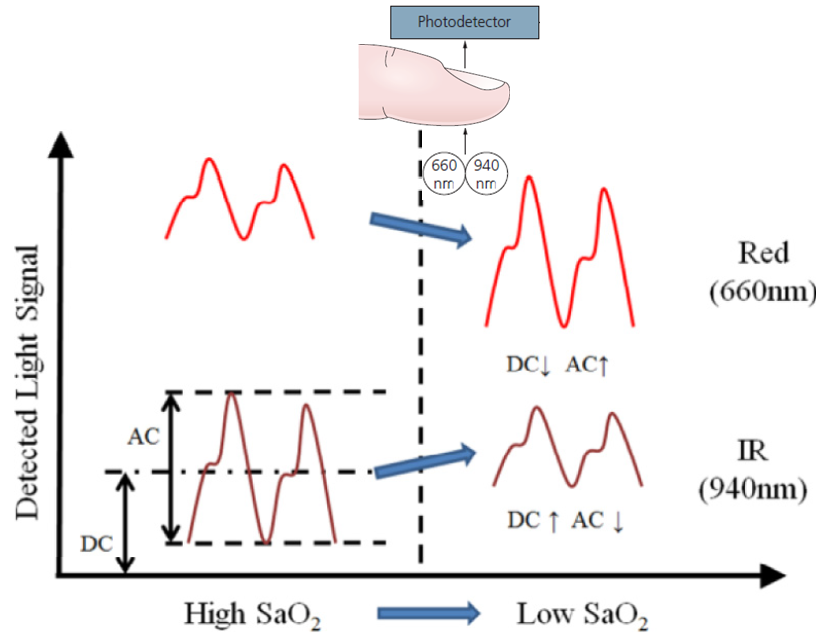
\includegraphics[width=3in]{principio_funcionamiento.png}
	\caption{Principio de funcionamiento del oximetro de pulso, editado de \cite{B_reflectance_pulse_oximetry}. }.
	\label{principio_funcionamiento}
\end{figure}


En cuanto al telemonitoreo de estas variables, internet permite incorporar diferentes herramientas de software que envian la información a servidores web y permiten su visualización en diferentes dispositivos.  Estas aplicaciones se pueden dividir en dos partes: la aplicación que recibe la información del elemento sensor (en este caso el oxímetro de pulso) y que permite el acceso a la base de datos; y la aplicación que permite la visualización de la información por parte del cliente.

El presente artículo aborda la telemetría de la saturación de oxígeno con la respectiva evaluación de resultados en perspectiva de aplicaciones futuras en telemedicina. En la sección 2 se presentan los elementos usados para la elaboración del oxímetro de pulso, envío y recepción de información; en la sección 3 se presenta la implementación de herramientas de procesamiento de señales para la medición de saturación de oxígeno y frecuencia cardíaca, así como el diseño del software asociado a la aplicacion web; en la sección 4 se exponen los resultados obtenidos de la aplicación en conjunto; para finalizar con las conclusiones  de la implementación desarrollada en la sección 5.










\section{Materiales}

{\color{blue}D}
Para adquirir la señales que permitan la medición de saturación parcial de oxígeno y de frecuencia cardíaca se hace uso del módulo sensor con referencia MAX30102 que incluye los leds y fotodetectores descritos en la figura \ref{principio_funcionamiento} más elementos ópticos y electrónicos de bajo ruido. Las señales adquiridas por el sensor, y mostradas en la figura \ref{principio_funcionamiento} (pletimsografía en rojo e infrarrojo), son enviadas mediante interfaz I2C a un  módulo microcontrolado de referencia ESP32. Este módulo incluye la funcionalidad de conexión wifi para enviar la información procesada a un servidor web;  la información enviada se compone de  la señal de pletismografía de infrarrojo (señal que en términos generales se ve menos afectada por ruido), junto con los valores resultantes de saturación parcial de oxígeno y frecuencia cardíaca. Adicionalmente, la información es visualizada también en una pantalla OLED de 1.3'' dada la comunicación I2C con el módulo microcontrolado. En conjunto, estos elementos se presentan gráficamente en la figura \ref{materiales}.
  


\begin{figure}[!h]
	\centering
	\includegraphics[width=3in]{Materiales.png}
	\caption{Materiales usados en la implementación.}
	\label{materiales}
\end{figure}



%Para la evaluación de desempeño de los algoritmos de reconocimiento automático de patrones en la detección de fibrilación auricular en computador de placa reducida se propone el uso de la base de datos MIT-BIH AFIB (encontrada en \cite{physiobank}). Base de datos de uso generalizado en investigaciones afines y que contiene 23 registros de electrocardiografía de pacientes que presentan fibrilación auricular, con una frecuencia de muestreo de 250Hz, a una resolución de 12 bits y un rango de $+/-10mv$. Cada registro tiene una duración de 10 horas, en total se incluyen 291 episodios de fibrilación auricular con un tiempo promedio de 115 segundos, y 344 episodios de otros ritmos cardíacos \cite{wavelet_svm_afib}. Estos episodios se encuentran marcados, con anotaciones en tiempos específicos según revisiones previas de especialistas creadores de la base de datos; en la figura \ref{imagen_ecg} se representa un ejemplo de un archivo de la base de datos con la anotación respectiva en la medida que la señal cardíaca cambia llegando el segundo 5 de ritmo normal a ritmo con fibrilación auricular.

%\begin{figure}[!h]
%	\centering
%	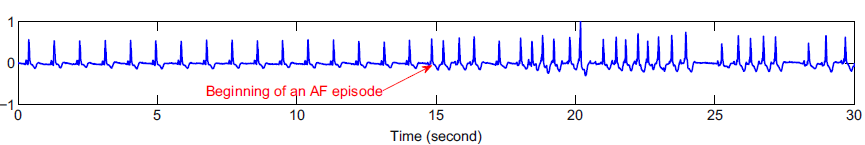
\includegraphics[width=3.5in]{base_datos_archivo.png}
%	\caption{Ejemplo de lectura de señal filtrada en archivo 4048 MIT-BIH AFIB con su anotación respectiva, tomado de \cite{wavelet_svm_afib}
%	}.
%	\label{base_datos_archivo}
%\end{figure}


%El sistema a utilizar consta de un computador de placa reducida Raspberry Pi 2 (que cuenta con un procesador quad-core ARM Cortex-A7, 1 GB de memoria RAM y puertos digitales para comunicación con diferentes periféricos \cite{rpi2}). En él se realiza el preprocesamiento, la extracción de características y el reconocimiento automático de fibrilación auricular de señales tanto guardadas en memoria como provenientes del módulo análogo digital externo ADS1115 (conversor con resolución de 16 bits y frecuencia de muestreo de 860Hz) conectado vía I2C y que permite adquirir la señal a analizar preveniente de un generador de señales. Una vez los algoritmos son ejecutados, la información es almacenada en memoria y es presentada en una pantalla TouchScreen referencia ADAFR-2097 para visualizar tanto la señal analizada como el resultado de su análisis. En la figura \ref{hardware} se representa el hardware implementado.






\section{Métodos}


{\color{blue}B E}


La temería de la saturación de oxígeno en sangre y la frecuencia cardíaca implica, en primera instancia, la adquisición de las señales de pletismografía en rojo e infrarrojo presentadas de manera conceptual en la figura \ref{principio_funcionamiento}, estas señales entregadas por el módulo sensor MAX30102 son leídas por el módulo microcontrolado ESP32 para que una vez procesadas se realice el envío de la información al servidor. A continuación se presentan los métodos asociados al módulo microcontrolador (adquisición, procesamiento y envío de la información al servidor), posteriormente se presentan los métodos relacionados con el servidor (recepción de la información y su visualización en aplicación web).

\subsection{Adquisición, procesamiento y envío de información.}
A las señales en rojo e infrarrojo leídas por el módulo ESP32, después del filtrado digital adecuado, se les pueden extraer ciertas características simples a utilizar en el cálculo de la saturación de oxígeno. El valor R determina la relación normalizada entre la señal en rojo versus la señal en infrarrojo (ver ecuación \ref{ecuación_R} y figura \ref{principio_funcionamiento}) y con este valor se puede estimar la saturación de oxígeno mediante la aproximación lineal que se presenta en la ecuación 2 \cite{E_FFT_Spo2}. 

\begin{equation}
	R=\frac{AC_{rojo}/DC_{rojo}}{AC_{infrarrojo}/DC_{infrarrojo}}
	\label{ecuación_R}
\end{equation}

\begin{equation}
	SpO_2 = 110-25R
	\label{ecuación_SpO2}
\end{equation}


El problema principal radica en realizar al tratamiento adecuado de señales para obtener un valor R dependiente sólo de la saturación arterial de oxígeno del paciente. Paralelo a esta medición se puede estimar la frecuencia cardíaca (de la señal en infrarrojo); para así realizar el envío de la información al servidor. 

Con el módulo microcontrolado ESP32, dada la alta demanda de recursos computacionales, se abordó este problema mediante la implementación de tres tareas concurrentes que se describen en la figura \ref{Descripción_firmware}. Una tarea se destinó a la lectura de los datos almacenados en el sensor, con el acceso a los buffers de la señal infraroja y roja; adicionalmente, esta tarea permitió la actualización permanente de la intensidad de los led asociados, contrarrestando las fluctuacinoes en la cantidad de luz ambiental. Por otra parte, una tarea adicional se destinó al procesamiento de la señales adquiridas para aplicar la ecuación \ref{ecuación_R} y \ref{ecuación_SpO2}. Esta información es utilizada por la tarea 3 para ser enviada de manera organizada al servidor web.


\begin{figure}[!h]
	\centering
	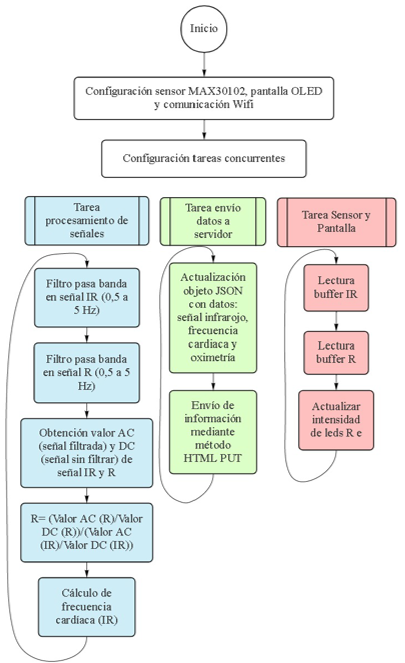
\includegraphics[width=3.5in]{diagrama_flujo.png}
	\caption{Descripción de firmware. Las siglas IR corresponden a la abreviatura de infrarojo, mientras que R hace referencia a rojo}.
	\label{Descripción_firmware}
\end{figure}



Para optimizar las lecturas realizadas por el sensor se siguieron las recomendaciones de configuración establecidas en \cite{E_Recomended_configurations_MAX30102_maxim} \cite{E_SNR_MAX30102}. Mientras que para el procesamiento de la señal se usaron las frecuencias de corte de filtrado y el método de calculo de valores AC y DC estudiado en \cite{E_FFT_Spo2}; para calcular los valores AC se implementó el cálculo de la densidad espectral de potencia, como se sugiere en \cite{E_psd_ppg}.


\subsection{Telemetría}

{\color{blue}B F}


En cuanto a la necesidad de visualizar de manera remota los resultados obtenidos por el sistema embebido, se optó por el envío de la información vía internet, para lo cual el microcontrolador se conecta mediante Wifi al servidor web, como se describe en la figura \ref{materiales}. Este servidor  alberga código en Python para el acceso a la base de datos; y adicionalmente código en Javascript para la visualización de la información en tiempo real con el uso de librerías y de una planilla como en el desarrollo presentado en \cite{F_iot_spo2_wrist}. Los códigos se integraron en una sola aplicación en el framework Django, lo que no se logra con otros frameworks destinados específicamente bien sea al desarrollo de aplicaciones backend o frontend.

 

\section{Resultados}
{\color{blue}G}
Para la implementación del sistema embebido propuesto, en primera instancia se realizó una aplicación de escritorio con código en Python en el IDE de Spyder, como se muestra en la figura \ref{resultado_python_real}. Esta aplicación, que realizó la adquisición y procesamiento en tiempo real de las señales con el módulo ESP32 como tarjea de adquisición de datos, permitió depurar el código relacionado al procesamiento de señales (filtrado, cálculo de densidad espectral de potencia y determinación de oximetría y frecuencia cardíaca), antes de su migración al sistema embebido. El desempeño de la aplicación de escritorio fue el adecuado en cuanto a la eliminación de ruido, procesamiento en tiempo real y resultados acordes con los signos vitales del usuario del dispositivo.


\begin{figure}[!h]
	\centering
	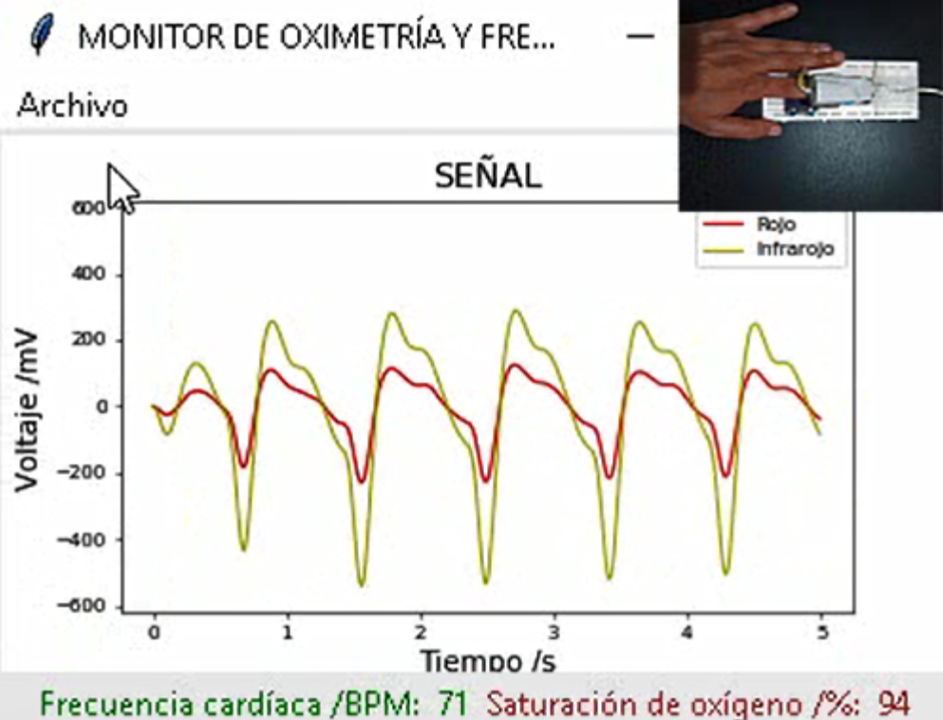
\includegraphics[width=2.5in]{resultado_python_real.png}
	\caption{Prueba funcional con aplicaciòn de escritorio en Python}
	\label{resultado_python_real}
\end{figure}


Una vez realizada la migración del código en Python a código en C++, se realizaron las pruebas del sistema embebido final que se muestra en la figura \ref{montaje_final}. Las pruebas funcionales fueron satisfactorias en términos de la ejecución en tiempo real por la implementación de las tareas en paralelo descritas en la figura \ref{Descripción_firmware}. Los resultados fueron los mismos obtenidos en la aplicación de escritorio, con pequeñas variaciones en los resultados que fueron eliminadas luego de realizar la importación de los coeficientes de los filtros con las suficientes cifras significativas (10).

\begin{figure}[!h]
	\centering
	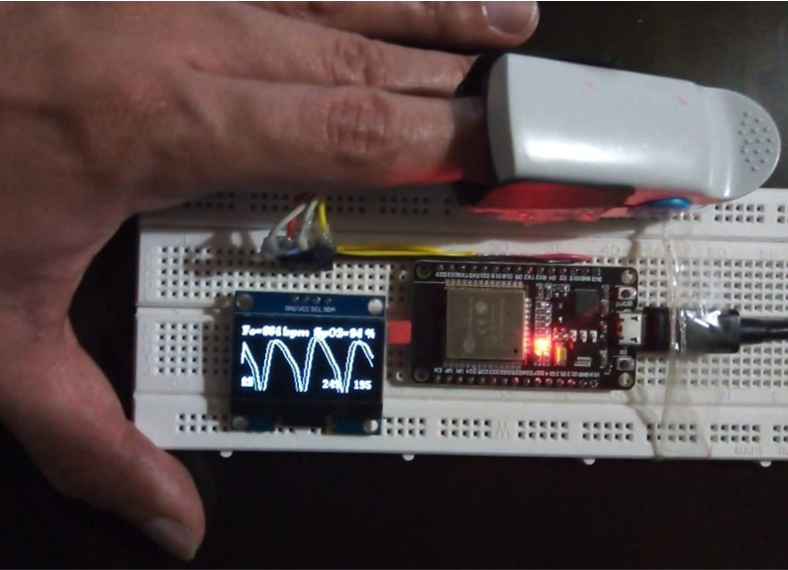
\includegraphics[width=2.5in]{montaje_final.png}
	\caption{Montaje}
	\label{montaje_final}
\end{figure}

Con respecto a las mediciones para validar el funcionamiento del oxímetro en diferentes valores, si bien en el mercado existen dispositivos que comúnmente se conocen como simuladores, según \cite{G_There_is_no_such_thing_as_a_SpO2_simulator} los dispositivos actuales solo pueden interpretarse como emuladores que imitan, con elementos optoelectrónicos, las valores de transmitancia para ciertas marcas comerciales. Y si bien se tiene la posibilidad de configurar una nueva marca o hacer variaciones sobre las existentes, se trata de dispositivos diseñados para probar sensores transmisivos \cite{G_validacion_oximetro_texas_fluke} mas no reflectivos, como es el caso del sensor MAX30102.

Con el propósito de poner a prueba el sistema embebido en términos del estimativo de la saturación parcial de oxígeno, se realizó un comparativo con un oxímetro de pulso comercial de marca AccuMed modelo Cms-50d1; los resultados, que incluyeron la participación de 3 individuos en condiciones tanto normales, como de hipo e hiperventilaciòn, 
%, se encuentran en la figura \ref{resultado_comparacion_oximetro}
demostraron una correlación entre las dos variables de $r=0.87$ para saturaciones entre $88\%$ y $97\%$ (14 parejas de datos). 
%Al respecto, existe una gran dificultad en la obtención de estos datos dado que se tienen tiempos de respuesta diferentes entre los dispositivos que se comparan. 
En la medida que se observa una relación lineal entre las mediciones de los dos dispositivos, se espera un comportamiento similar en saturaciones más bajas, lo cual puede ser validado con la inhalación controlada de una mezcla pobre en oxígeno como se plantea en \cite{G_validacion_sensor_maxim}.


%\begin{figure}[!h]
%	\centering
%	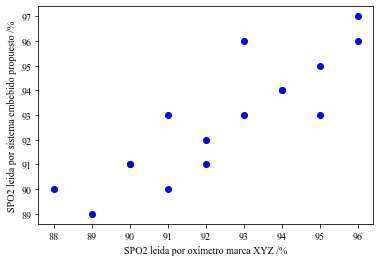
\includegraphics[width=3in]{resultado_comparacion_oximetro.png}
%	\caption{Prueba funcional de aplicaciòn Web}
%	\label{resultado_comparacion_oximetro}
%\end{figure}


Finalmente, en la figura \ref{resultado_aplicacion_web} se presenta la captura de pantalla del funcionamiento, en un explorador web, de la aplicación creada para el telemonitoreo. Se observó el despliegue en tiempo real tanto de la señal como de los valores de SPO2 y frecuencia cardíaca, lo que implica la posibilidad de monitorizar otros signos vitales e incluir herramientas computacionales adicionales en la misma plataforma.

\begin{figure}[!h]
	\centering
	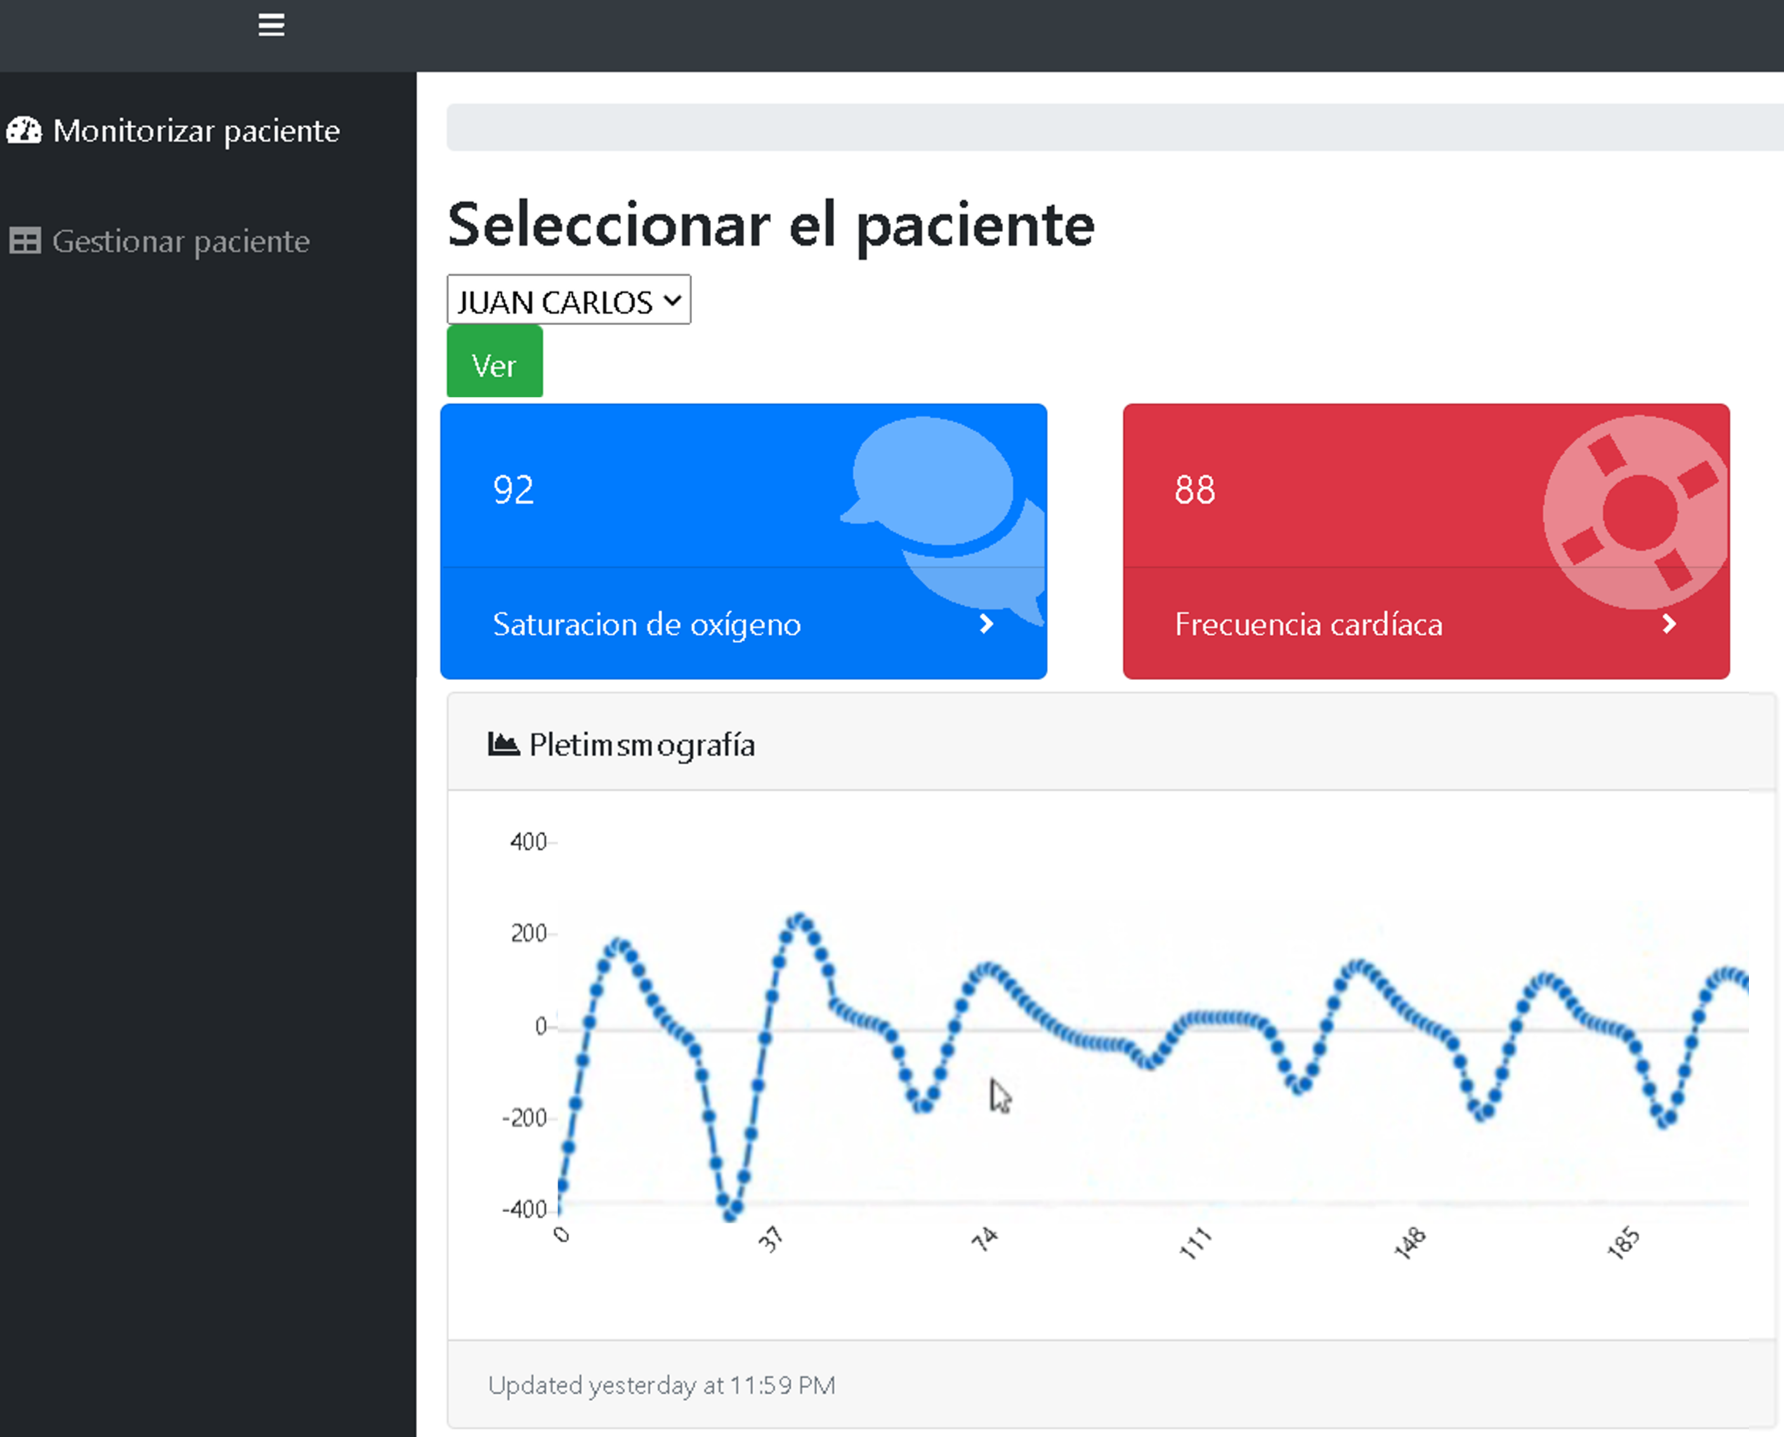
\includegraphics[width=3in]{resultado_aplicacion_web.png}
	\caption{Prueba funcional de aplicación Web, la señal corresponde a la pletismografia en infrarojo; los recuadros en azul y rojo presentan el valor de SPO2 y la frecuencia cardíaca, respectivamente}
	\label{resultado_aplicacion_web}
\end{figure}


%	\begin{table}[h!]
%		\centering
%		
%		\caption{Resultados obtenidos error e incertidumbre
%		}
%		%\cite{ica_bayes_gmm_afib} }
%		\def\arraystretch{1.2}%  controla padding
%		\begin{tabular}{c c l}
%			%		\toprule
%			
%			\hline
%			\textbf{Tecnología} & \multicolumn{1}{c}{\textbf{Error}} & \textbf{Incertidumbre}	\\ 
%			\hline
%			Nellcor  &--	& --\\
%			%\hline
%			Massimo  &--	& --\\		
%	
%			
%			\hline
%			%\bottomrule
%		\end{tabular}%
%		\label{cuadro:resultados_sn_sp}%
%	\end{table}%




\section{Conclusiones}


La implementación de un sistema de telemonitoreo de oximetría de pulso requiere el uso de algoritmos de procesamiento digital de señales y de envío permanente de la información procesada, lo que con microcontroladores actuales debe abordarse con la ejecución en paralelo de diferentes tareas en garantía del procesamiento y envío en tiempo real de la información.


Uno de los principales retos en el desarrollo de oxímetros de pulso se relaciona con el filtrado de las señales de pletismografìa; en la medida que de esto depende que el cálculo del valor R se relacione adecuadamente con la oximetría del usuario del dispositivo y en rechazo de artefactos propios del uso de los elementos optoelectrónicos involucrados. Es por ello que resulta conveniente utilizar de manera previa un computador personal como sistema de procesamiento de señales en tiempo real, para así realizar el diseño de filtros y de funciones del cálculo del valor R, y seguidamente realizar la migración de código al sistema embebido. Esto posibilita incluso explorar herramientas más robustas, como las de inteligencia artificial, para mejorar el desempeño de los algoritmos \cite{E_spo2_wrist_machine_learning}.

El cálculo de la densidad espectral de potencia de las señales de pletismografìa, permite una adecuada estimación de las variables involucradas en el cálculo del valor R y la consecuente determinación correcta de la saturación parcial de oxígeno. El desempeño de estas funciones, en conjunto con los algoritmos implementados en el servidor web, dan cuenta de la posibilidad de integrar más signos vitales y usuarios de dispositivos para el telemonitoreo con miras al desarrollo de plataformas de telemedicina.




 






\bibliography{mis_referencias}
\bibliographystyle{IEEEtranN}

\end{document}